% =====================================================================
%  CHAPTER 6 - TESTING AND EVALUATION METHOD
% =====================================================================
\clearpage
\chapter{Testing and Evaluation Method}

The engine was tested at four levels: unit tests of individual packages,
integration tests against a real PostgreSQL instance, fault-injection tests at
named crash points, and end-to-end tests on a local three-node cluster. It was
then evaluated on a cluster in Amazon Web Services. This chapter describes the
tests and the local results, and then the cloud test bed and the measurement
procedure whose results are reported in Chapter~7.

\section{Unit and Integration Tests}

The suite contains 597 test functions, which expand to 1,229 test cases when
table-driven subtests are counted. Table~\ref{tab:tests} gives their
distribution. Tests that need a database start a disposable PostgreSQL
schema through the \cd{testdb} helper, so the storage code is never tested
against a mock. Three groups of tests carry most of the weight for
correctness.

\begin{enumerate}[leftmargin=*, itemsep=2pt]
  \item \emph{Ownership.} The pure \cd{Decide} and \cd{Apply} functions of
    the lease manager are tested over all combinations of lease state,
    renewal outcome and elapsed time. Integration tests run two lease
    managers against one database and check that a shard never has two
    owners whose tokens are both accepted.
  \item \emph{Fencing.} A commit is attempted with a stale token for each
    kind of write (start, decision, timer, signal) and the test checks that
    nothing from the transaction is visible afterwards.
  \item \emph{Replay.} Workflows are run, interrupted at each call position
    and re-executed against the stored history; the result must be identical
    and no activity may be scheduled twice. Changed workflow code must be
    reported as a non-determinism error.
\end{enumerate}

\begin{table}[htbp]
  \centering
  \caption{Distribution of test functions by package}
  \label{tab:tests}
  \small
  \begin{tabular}{|l|r|l|r|}
    \hline
    \textbf{Package} & \textbf{Tests} & \textbf{Package} & \textbf{Tests} \\
    \hline
    \cd{runtime}  & 70 & \cd{eventlog} & 20 \\
    \hline
    \cd{api}      & 59 & \cd{config}   & 18 \\
    \hline
    \cd{workflow} & 33 & \cd{faultinj} & 15 \\
    \hline
    \cd{taskq}    & 32 & \cd{timers}   & 14 \\
    \hline
    \cd{lease}    & 31 & \cd{obs}      & 13 \\
    \hline
    \cd{activity} & 25 & \cd{saga}     & 10 \\
    \hline
    \cd{shard}    & 21 & others        & 236 \\
    \hline
    \multicolumn{3}{|l|}{Total test functions (test cases including subtests)} &
      597 (1,229) \\
    \hline
  \end{tabular}
\end{table}

\section{Fault Injection at Crash Points}

The \cd{faultinj} package defines six named crash points, armed by an
environment variable: \cd{BeforeStartCommit}, \cd{BeforeDecisionCommit},
\cd{BeforeResultJournal}, \cd{AfterActivityJournaled},
\cd{BeforeNextPlanCompletes} and \cd{AfterLeaseRenew}. When the armed point is
reached, the code returns an error at that boundary and the transaction in
progress is abandoned. Three of the points were exercised on a local
Kubernetes cluster by a script that arms the point, restarts the engines,
drives a workflow through the boundary and inspects the database. A start
abandoned at \cd{BeforeStartCommit} left no execution row and was admitted
cleanly on retry. A decision abandoned at \cd{BeforeDecisionCommit} in the
middle of a run, with three activities already recorded and a timer
pending, was retried; the run completed with four scheduled and four
completed activities and no duplicate event. A crash at
\cd{AfterActivityJournaled} likewise produced no duplicate (run, sequence
number) or program-order position. The remaining points are covered by unit
tests. These seams test the boundary of durable state; loss of a
whole process was tested separately by killing processes, both locally and on
the cloud test bed.

\section{Local Cluster Tests}

A Docker Compose cluster of three engine nodes was used to test behaviour
that needs real processes. The most direct test is the duplicate audit: 1,000
delivery workflows were started at a concurrency of 64 while one node was
killed after 8\,s and a second 12\,s later, and both were restarted while the
batch was running. 763 runs completed. The remaining 237 starts were refused
with \cd{NotOwner} while their shards had no owner; they were never accepted
and so were never at risk. An audit of the 3,052 recorded activity completions
found no duplicate (shard, workflow, run, $k$), and every accepted run ended in
the \cd{COMPLETED} state. A promotion drill with a streaming standby database
was also carried out locally, but the cloud evaluation used a single database
host and the drill is not discussed further.

The duplicate check was evaluated offline on four corpora of request pairs,
all built the same way: several phrasings of one action form duplicate
pairs, and phrasings of two actions that differ in one deciding detail form
distinct pairs. The flight corpus has 213 pairs (98 duplicate). Three
further corpora have 300 pairs each, 15 duplicate and 15 distinct per kind
of task: a development corpus of ten kinds (flight, payment, refund,
meeting, message, order, provisioning, ticket, subscription, shipment) and
two held-out corpora of ten kinds each (hotel, car rental, share trade,
insurance claim, password reset, file sharing, payroll, DNS change,
prescription, deployment; and cab, invoice, leave, bill payment, event
tickets, backup, access grant, table booking, repair, funds transfer). Each
held-out corpus was committed to the repository before the comparator
version it was used to test, and was scored once. A fifth set holds 45
genuine rewordings produced by a live language model on both sides of a
simulated crash; it has no distinct pairs. Labels follow from the
construction and were not assigned by human annotators.

\section{Cloud Test Bed}

The cloud evaluation ran on the infrastructure shown in
Fig.~\ref{fig:testbed}, in one availability zone of the \cd{us-east-1} region.
Three engine pods ran on three m7i-flex.large nodes, one pod per node, with
the default configuration of 16 shards, four workflow workers and eight
activity workers per shard. PostgreSQL~16 ran on a separate m7i-flex.large
host with \cd{synchronous\_commit} on and no standby. The load generator ran
on a separate, tainted node so that it competed with nothing. All commands
were issued from an operator instance inside the VPC, reached through AWS
Systems Manager, and every result file was copied to S3 with its command line,
image digest and harness version.

\begin{figure}[htbp]
  \centering
  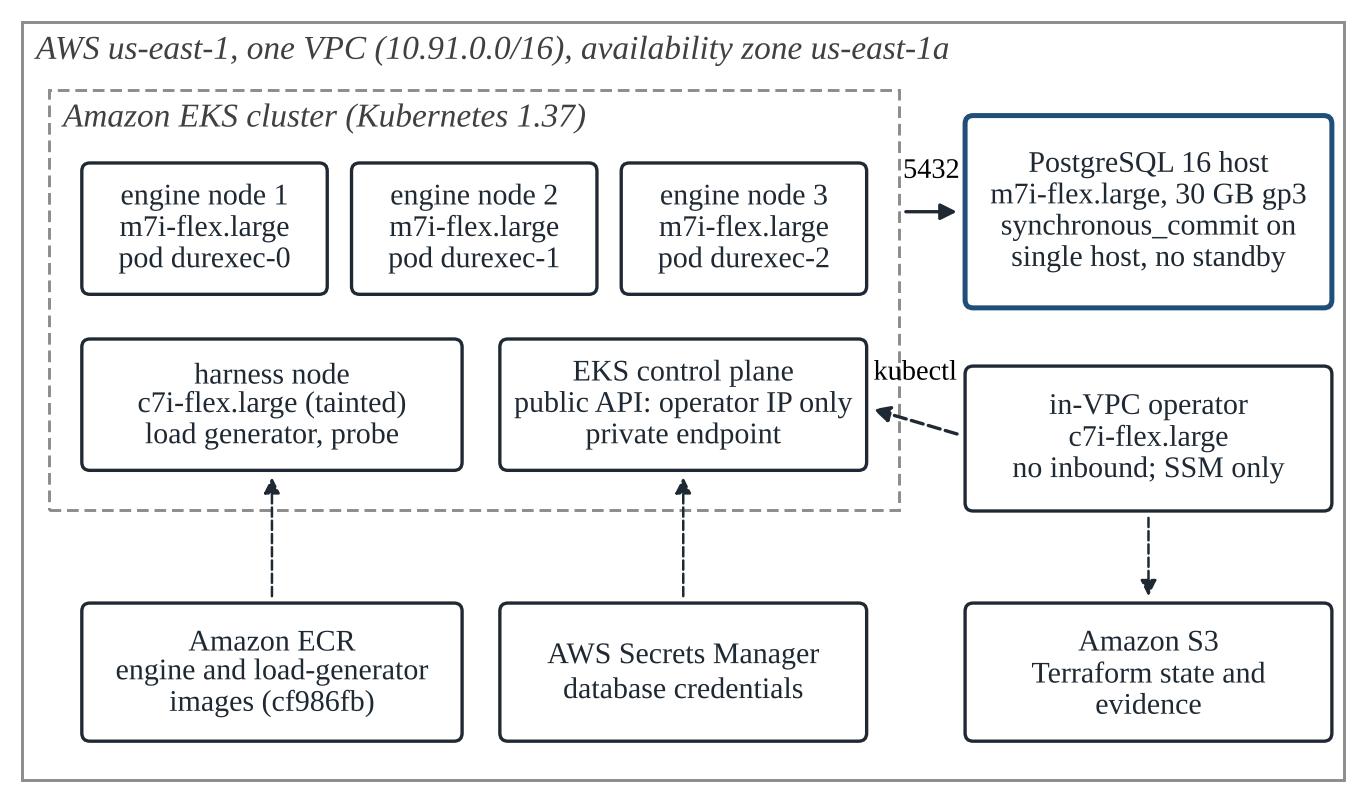
\includegraphics[width=0.92\linewidth]{figures/fig_6_1_aws_testbed.png}
  \caption[Cloud test bed on AWS]{Cloud test bed on AWS.}
  \label{fig:testbed}
\end{figure}

\section{Measurement Procedure}

The load generator starts delivery workflows and records the time from the
start request to completion. It runs in one of two modes, following the
distinction drawn by Schroeder \emph{et al.}~\cite{openclosed2006}. In
\emph{closed-loop} mode, $c$ clients each start a new workflow when their
previous one completes, so the arrival rate falls when latency rises. In
\emph{open-loop} mode, workflows are started at a fixed rate regardless of
completions, which is how independent users behave. By Little's
law~\cite{little1961}, a closed loop with $c$ clients and latency $W$ carries
$c/W$ workflows per second, so closed-loop throughput can look stable even
when the system is overloaded. Both the median and the 99th percentile are
reported, because in a system of many cooperating parts it is the tail that
determines the experience of users~\cite{tailatscale2013}.

Each measurement point ran for 135\,s, of which the first 15\,s were
discarded as warm-up; the calibration points ran for 435\,s to collect
enough samples. Table~\ref{tab:stages} lists the stages. Ladder stages
screened a range of concurrencies with one trial each and then repeated the
best two with three trials; the knee was chosen from the means of the
repeats, not from the screen, because single trials near saturation were
found to vary by up to 40\%.

\begin{table}[htbp]
  \centering
  \caption{Evaluation stages}
  \label{tab:stages}
  \small
  \begin{tabular}{|p{0.28in}|p{1.65in}|p{3.26in}|}
    \hline
    \textbf{Stage} & \textbf{Purpose} & \textbf{Procedure} \\
    \hline
    B & Idle overhead & No workload; database commits per second for five
      configurations, 3 trials each \\
    \hline
    C & Latency floor & Closed loop at $c=1$, and open loop at 1\,wf/s,
      3 trials each \\
    \hline
    D & Closed-loop capacity & $c$ from 4 to 512; repeats at 128, 256, 512 \\
    \hline
    E & Open-loop capacity & 0.5 to 1.1 times the Stage~D knee, 3 trials each \\
    \hline
    F & Worker sensitivity & Workers per shard 2+4 and 8+16 against the
      default 4+8 \\
    \hline
    G & Shard sensitivity & 32 and 64 shards at a constant 192 workers \\
    \hline
    H & Replica scaling & One and two engine replicas against three \\
    \hline
    Faults & Recovery & Six fault types under open-loop load
      (Section~\ref{sec:faultmethod}) \\
    \hline
    M1 & Workflow types & Each of six types alone, $c=32$ \\
    \hline
    M2--M3 & Mixed capacity & Six-type mix: $c$ from 32 to 256 with repeats; open
      loop at 40--100\,wf/s \\
    \hline
    M4 & Mixed faults & Process kill and 35\,s freeze under the mix \\
    \hline
  \end{tabular}
\end{table}

Every point was classified by the harness before it was accepted. A point was
\cd{RECORDED} if the generator itself was not a bottleneck (its CPU, lag and
in-flight count were checked) and every started workflow completed. A point
with failed or unfinished runs was marked for correctness review, and one in
which the generator could not keep up was marked invalid and excluded. After
every point, a set of SQL invariants was run over the journal: no duplicate
(run, sequence number), no duplicate activity completion, no completion
without a matching schedule, no gap in sequence numbers and no run with more
than one terminal event. During each point the harness also sampled the CPU
of every node, the database's commit rate, WAL throughput, wait events and
lock waits, and the engines' connection-pool statistics.

\section{Fault-Injection Procedure}
\label{sec:faultmethod}

Each fault trial ran an open-loop load of 65.6 workflows per second, half the
closed-loop knee and a rate sustained without loss in Stage~E, and injected
one fault after the load had settled, in the manner of chaos engineering
experiments on production systems~\cite{chaos2016}. Six faults were used, each with three
trials on a different victim pod, except the database reboot, which was run
once:

\begin{enumerate}[leftmargin=*, itemsep=1pt]
  \item graceful deletion of an engine pod;
  \item \cd{SIGKILL} of the engine process;
  \item freezing the engine process with \cd{SIGSTOP} for 35\,s, longer than
    the 10\,s lease, then resuming it;
  \item severing the engine's database connections;
  \item draining the Kubernetes node that hosts an engine pod;
  \item rebooting the database host.
\end{enumerate}

\begin{figure}[htbp]
  \centering
  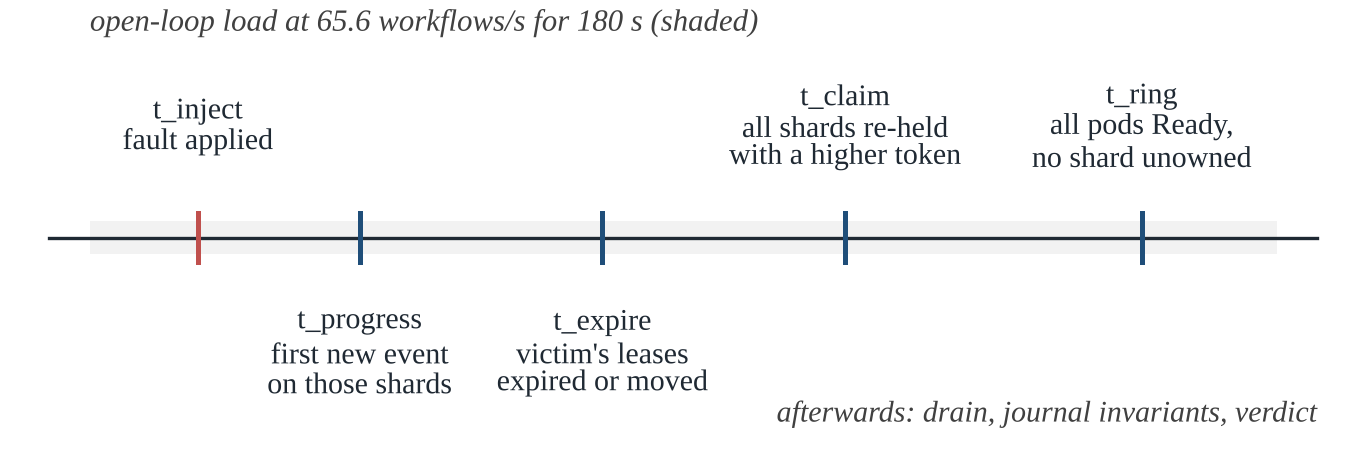
\includegraphics[width=0.92\linewidth]{figures/fig_6_2_fault_timeline.png}
  \caption[Timing of a fault trial]{Timing of a fault trial. All times are
    measured from injection on the PostgreSQL clock.}
  \label{fig:faulttimeline}
\end{figure}

The recovery of each trial was measured on the database clock, from the
moment of injection, by polling the lease table and the event log
(Fig.~\ref{fig:faulttimeline}). $t_\text{expire}$ is the time at which the
victim's leases expired or moved; $t_\text{claim}$ the time at which all of
them were held again with a higher fencing token; $t_\text{progress}$ the time
of the first new event on those shards; and $t_\text{ring}$ the time at which
all pods were ready and no shard was unowned. The fencing-rejection counters
of all engines were read before and after, and the journal invariants were
checked after the load had drained. A trial was valid only if the cluster was
healthy before injection and the injection was confirmed to have happened;
early attempts that failed these checks because of harness defects were kept
in the results file as invalid and are not counted.
